\documentclass[
a4paper,   
headsepline, 
fleqn,     
12pt
]{scrartcl}

%%% ngerman: language set to new-german
\usepackage{ngerman}
\usepackage[latin1]{inputenc}
\usepackage[T1]{fontenc}
\usepackage{ae,aecompl}

%%% Graphic stuff
\usepackage{graphicx}
\usepackage{amsmath,amssymb,amstext}
\usepackage{units}
\usepackage{scrpage2}

\setlength{\parindent}{0em} 

\newcommand{\mygraphics}[3]{
  \begin{center}
    \includegraphics[width=#1, keepaspectratio=true]{#2} \\
    \textbf{#3}
  \end{center}
}

%%%      footer - middle: page number
\pagestyle{scrheadings}

%%% heading - left
 \ihead[]{Marco Sohm, Kevin Wallis}

%%% heading - right
 \ohead[]{Aufgabe 1}

\begin{document}

 \pagenumbering{roman} %% small roman page numbers
 \pagenumbering{arabic} 

\subsection*{Erweiterung des Vorlesungsbeispiels}
Abh�ngig vom gew�hlten $C_{start}$ sind unterschiedliche Verhalten in der Simulation erkennbar. Bei der Simulation wurde $C_{start}=0$ festgelegt dadurch ist ersichtlich, dass sich der C Wert der beiden Schichten erh�ht und ab einem bestimmten Zeitpunkt (ca. $2000$ ZE (Zeiteinheiten, Wochen)) konstant bleibt. Das es sich hierbei um ein Gleichgewicht handelt, wird im Abschnitt \textit{Berechnen des Gleichgewichtszustands} genauer erl�utert. 

\subsection*{Berechnen des Gleichgewichtszustands}
Im Folgenden werden die beiden Gleichungen f�r $\frac{dC_E}{dt}$ und $\frac{dC_H}{dt}$ angegeben.

\begin{itemize}
\item $\frac{0.34*1e6 * 320}{50*1e6} + \frac{C_H * 0.5*1e6}{50*1e6} - \frac{0.34*1e6 * C_E}{50*1e6}-0.02 * C_E- \frac{0.5*1e6 * C_E}{50*1e6} = 0$
\item $\frac{0.5*1e6 * C_E}{100*1e6}-0.002 * C_H- \frac{0.5*1e6 * C_H}{100*1e6} = 0$
\end{itemize}

Aus der zweiten Gleichung kann $C_H$ wie folgt berechnet werden: $C_H = 5 * \frac{C_E}{7}$. Dieses Resultat wird in die erste Gleichung eingesetzt. Dadurch ergibt sich die folgende Gleichung:
$\frac{0.34*1e6 * 320}{50*1e6} + \frac{5 * C_E * 0.5*1e6}{7 * 50*1e6} - \frac{0.34*1e6 * C_E}{50*1e6}-0.02 * C_E- \frac{0.5*1e6 * C_E}{50*1e6} = 0$
Das Umstellen dieser Gleichung ergibt $C_E=73.372$. Dieser Ergebnis wird wiederum in das zuvor berechnete $C_H$ eingesetzt, somit ist $C_H=52.409$. Diese Werte wurden mithilfe der Simulation �berpr�ft (Siehe \ref{fig:Gleichgewicht}).\\

Ist das Gleichgewicht stabil? Ja, da das Gleichgewicht bei diesem Beispiel ein Attraktor ist. Dies wurde anhand von Events in der Simulation getestet. Ein Teil der Resultate sind im Anhang beigef�gt (Siehe \ref{fig:Attraktor} und \ref{fig:Attraktor_1}). Weitere Tests mit �ndern der C-Werte von Epilimnion und Hypolimnion wurden durchgef�hrt, jedoch dem Anhang nicht beigef�gt.

\subsection*{Zwischenschichtenmodel f�r den Winter}
Was kann man bez�glich des Gleichgewichts im Vergleich zum vorherigen Zwischenschichtenmodel sagen? Abh�ngig vom gew�hlten $k_R$ im Winter sehen die Simulationsergebnisse anders aus. Da in der Aufgabenstellung keine Angaben in Bezug auf das zu w�hlende $k_R$ vorhanden war, wurden beide Werte simuliert (Siehe \ref{fig:Stationaer_Sommer_Winter_kRE} und \ref{fig:Stationaer_Sommer_Winter_kRH}). Unabh�ngig vom gew�hlten $k_R$ ist das Ergebnis der Simulation periodisch oszillierend. Im Vergleich zum vorherigen Model ist es bei diesem Zwischenschichtenmodel nicht m�glich ein Gleichgewicht zu erreichen. Im Folgenden werden die Werte aus den beiden Simulationsergebnissen erl�utert.
\newline

\begin{tabular}{ l | l | l || l | l | l }
$k_{RE}$ Ab ca. 500 ZE station�r  & $C_{max}$ & $C_{min}$ & 
$k_{RH}$ Ab ca. 800 ZE station�r  & $C_{max}$ & $C_{min}$ \\
\hline
Epilimnion 		& 63.5 & 45 &	& 91 & 84 \\
Hypolimnion    	& 45 & 43.8 &	& 91 & 84 \\
Lake           	& 51 & 45 	&	& 91 & 84 \\
\end{tabular}

\newpage
\subsection*{Anhang}

\begin{figure}[h]
  \centering
  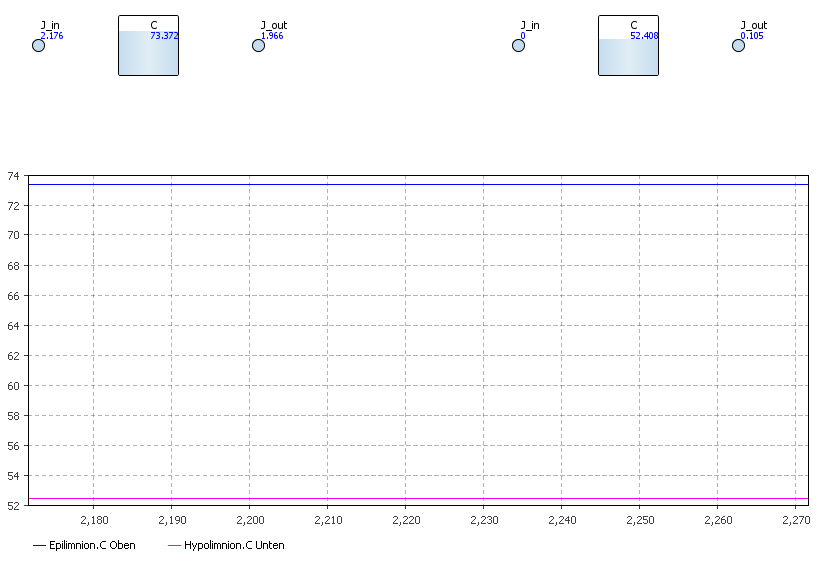
\includegraphics[width=1\textwidth]{./images/Gleichgewicht}
  \caption[Gleichgewicht: Simulation]{Simulation des Gleichgewichts}
  \label{fig:Gleichgewicht}
\end{figure}

\begin{figure}[h]
  \centering
  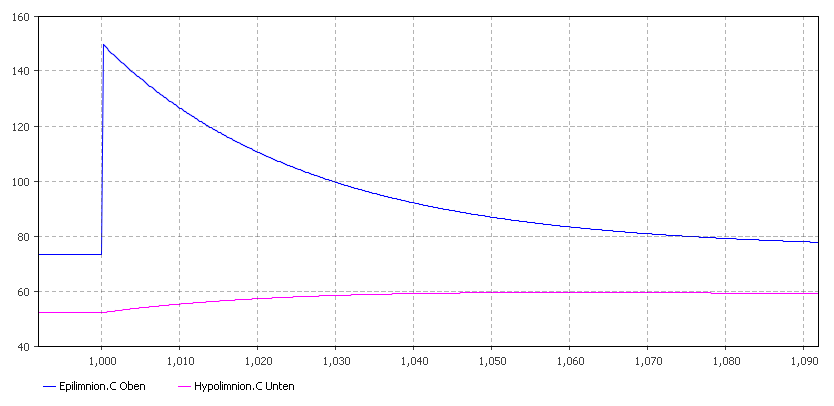
\includegraphics[width=1\textwidth]{./images/Gleichgewicht_Attraktor}
  \caption[Gleichgewicht: Simulation]{Simulation des Attraktors (C Epilimnion gr��er)}
  \label{fig:Attraktor}
\end{figure}

\begin{figure}[h]
  \centering
  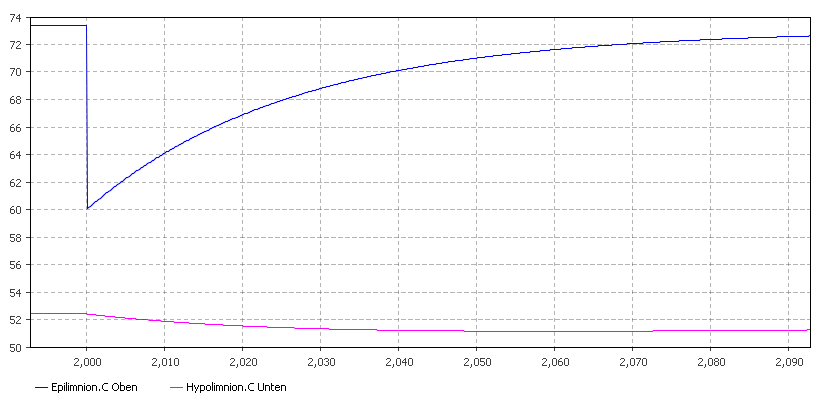
\includegraphics[width=1\textwidth]{./images/Gleichgewicht_Attraktor_1}
  \caption[Gleichgewicht: Simulation]{Simulation des Attraktors (C Epilimnion kleiner)}
  \label{fig:Attraktor_1}
\end{figure}

\begin{figure}[h]
  \centering
  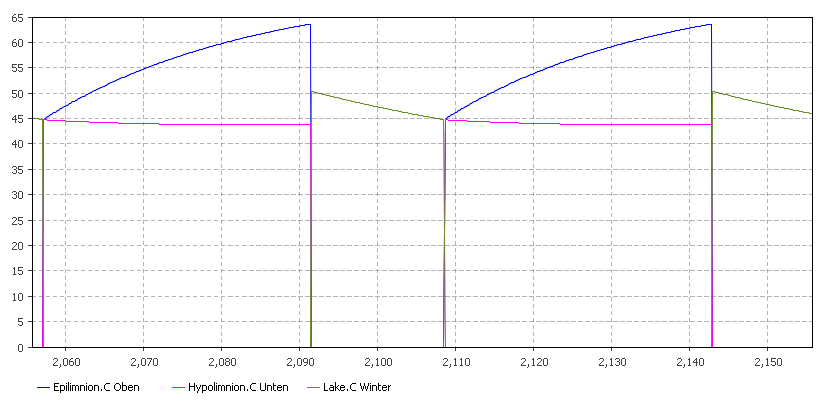
\includegraphics[width=1\textwidth]{./images/Stationaer_Sommer_Winter_kRE}
  \caption[Steady State: Simulation]{Steady State mit Sommer-Winter-�bergang $k_{RE}$}
  \label{fig:Stationaer_Sommer_Winter_kRE}
\end{figure}

\begin{figure}[h]
  \centering
  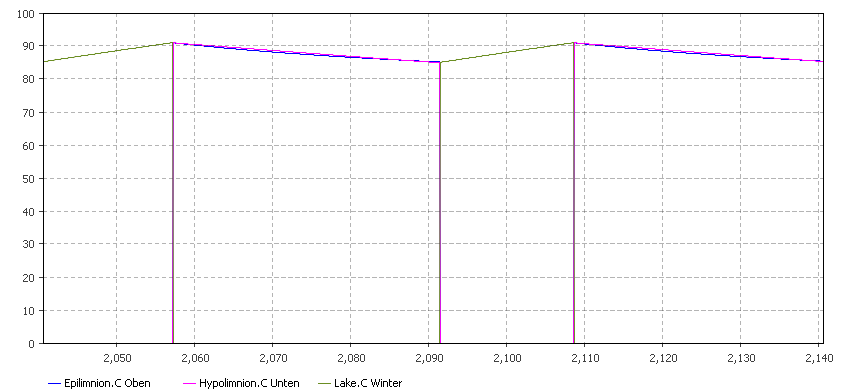
\includegraphics[width=1\textwidth]{./images/Stationaer_Sommer_Winter_kRH}
  \caption[Steady State: Simulation]{Steady State mit Sommer-Winter-�bergang $k_{RH}$}
  \label{fig:Stationaer_Sommer_Winter_kRH}
\end{figure}


\appendix  
\bibliographystyle{plain}
\bibliography{projekt.bib}

\end{document}